
\section*{Общая характеристика работы}

\newcommand{\actuality}{\underline{\textbf{\actualityTXT}}}
\newcommand{\progress}{\underline{\textbf{\progressTXT}}}
\newcommand{\aim}{\underline{{\textbf\aimTXT}}}
\newcommand{\tasks}{\underline{\textbf{\tasksTXT}}}
\newcommand{\novelty}{\underline{\textbf{\noveltyTXT}}}
\newcommand{\influence}{\underline{\textbf{\influenceTXT}}}
\newcommand{\methods}{\underline{\textbf{\methodsTXT}}}
\newcommand{\defpositions}{\underline{\textbf{\defpositionsTXT}}}
\newcommand{\reliability}{\underline{\textbf{\reliabilityTXT}}}
\newcommand{\probation}{\underline{\textbf{\probationTXT}}}
\newcommand{\contribution}{\underline{\textbf{\contributionTXT}}}
\newcommand{\publications}{\underline{\textbf{\publicationsTXT}}}


{\actuality} В~самых разнообразных и порой неожиданных академических, биофизических, технических геофизических приложениях исследователи сталкиваются с~проблемой массопереноса, инициированного волновым движением вдоль поверхности жидкости. Волновой массоперенос имеет самое непосредственное отношение к~проблемам расчета переноса загрязнения по поверхности океана; транспортировки примеси в~многослойных структурах, формирующихся как в~атмосфере, так и в~океане; к~вопросам моделирования закономерностей миграции некоторых видов флоры и фауны. Особый интерес исследователей связан с~переносом поверхностно--активных веществ (ПАВ) вдоль поверхности жидкости и влиянием плёнки ПАВ на~переносные свойства волн. В~связи с~этим не менее значимыми оказываются вопросы разработки методов мониторинга и управления местоположением областей загрязнения поверхности открытых водоемов и его влияния на~динамику волнового движения. Исследование влияния растворимых и нерастворимых плёнок ПАВ на~волновое движение на~поверхности жидкости тесно связано с~одной стороны с~перспективой формирования более полного понимания физической сути явления, а с~другой~--- для разработки новых методов управления условиями и характером протекания различного рода неустойчивостей, реализующихся на~поверхности жидкости.
 Несмотря на~давнюю историю вопроса и большое количество исследований в~этой области, в~практических приложениях дрейф, связанный с~волновым возмущением поверхности жидкости, учитывается при помощи модели, предложенной Дж.Г.~Стоксом еще в~середине XIX века. До сих пор не предложено простой аналитической, удобной для применения на~практике процедуры расчета скорости дрейфа Стокса в~многослойных системах жидкостей. В~начале XXI столетия активизировались экспериментальные и теоретические исследования в~области построения траекторий индивидуальных частиц жидкости, причем теоретические работы направлены в~основном на~использование численных методов расчета. 
\ifsynopsis

\else
Этот абзац появляется только в~диссертации.
Через проверку условия \verb!\!\verb!ifsynopsis!, задаваемого в~основном файле
документа (\verb!dissertation.tex! для диссертации), можно сделать новую
команду, обеспечивающую появление цитаты в~диссертации, но~не~в~автореферате.
\fi

% {\progress}
% Этот раздел должен быть отдельным структурным элементом по
% ГОСТ, но он, как правило, включается В~описание актуальности
% темы. Нужен он отдельным структурынм элемементом или нет ---
% смотрите другие диссертации вашего совета, скорее всего не нужен.

{\aim} данной работы является аналитическое асимптотическое исследование основных закономерностей волнового массопереноса в~идеальных и вязких жидкостях, а также изучение влияния тангенциального разрыва скоростей, поверхностного электрического заряда и плёнки поверхностно--активного вещества на~скорость дрейфа и характер движения индивидуальных жидких частиц, участвующих в~периодическом и переносном движениях.

Для~достижения поставленной цели были решены следующие {\tasks}:
\begin{enumerate}
  \item Разработана теоретическая аналитическая асимптотическая методика расчета траекторий движения индивидуальных частиц жидкости, участвующих в~волновом движении.
  \item Теоретическое аналитическое исследование влияния тангенциального разрыва скоростей на~границе раздела двух идеальных жидкостей на~закономерности движения индивидуальных жидких частиц и на~скорость массопереноса.
  \item Теоретическое аналитическое исследование влияния поверхностного электрического заряда на~закономерности движения индивидуальных жидких частиц и на~скорость массопереноса.
  \item Теоретическое аналитическое исследование влияния амплитудной модуляции волнового движения, оказываемое на~закономерности движения индивидуальных жидких частиц и на~скорость массопереноса.
  \item Теоретическое аналитическое исследование влияния плёнки поверхностно--активного вещества на~закономерности движения индивидуальных жидких частиц и на~скорость массопереноса в~вязких жидкостях.
  \item Теоретическое аналитическое исследование влияния волнового движения поверхности вязкой жидкости на~характер распределения поверхностно--активного вещества вдоль верхней границы жидкости.
\end{enumerate}


{\novelty}
\begin{enumerate}
  \item Впервые была разработана аналитическая асимптотическая методика расчета траекторий движения индивидуальных жидких частиц, участвующих в~волновом движении жидкости. Методика позволяет используя простые аналитические выражения построить траектории движения индивидуальных частиц жидкости с~учетом  факторов, оказывающих влияние на~круговую частоту волнового движения (например тангенциальный разрыв скоростей или поверхностный электрический заряд) и модулирующих амплитуду.
  \item Впервые было обнаружено новое явление неустойчивости Кельвина--Гельмгольца, заключающееся в~возникновении дрейфовых течений в~контактирующих жидкостях, направленных таким образом, чтобы уменьшить тангенциальный разрыв скоростей, инициировавший неустойчивость.
  \item Впервые аналитически во втором приближении по амплитуде волны описан характер движения индивидуальных жидких частиц в~присутствии поверхностно--активного вещества на~поверхности жидкости.
  \item Впервые аналитически было получено описание перераспределения  концентрации поверхностно--активного вещества, связанного с~волновым возмущением поверхности жидкости. Были получены зависимости положения максимума концентрации ПАВ от упругости плёнки.
  \item Впервые аналитически во втором приближении по амплитуде волны получены скорости дрейфового движения жидкости в~присутствии поверхностно--активного вещества на~её поверхности. Выделены составляющие дрейфового течения, связанные с~действием вдоль направления распространения волны горизонтальных вязких напряжений. 
\end{enumerate}

{\influence} работы состоит в~том, что полученные результаты представляют собой теоретическую основу для дальнейшего развития теоретических представлений о дрейфовых движениях, инициированных волновым движением вдоль поверхности жидкости, о траекториях индивидуальных жидких частиц, формирующих дрейфовое и циклическое движения, о характере перераспределения поверхностно--активных веществ вдоль поверхности жидкости. В~результате работы было обнаружено новое, неизвестное до этого явление неустойчивости Кельвина--Гельмгольца, которое представляет интерес для приложений,  имеющих дело с~системой двух жидкостей, испытывающих тангенциальный разрыв скоростей вдоль границы раздела. Полученные результаты по определению характера перераспределения плёнки ПАВ вдоль поверхности жидкости могут быть применены в~задачах мониторинга и прогнозирования распространения нефтяных разливов (и других поверхностно--активных веществ) в~мировом океане. В~работе развита новая методика расчета траекторий движения индивидуальных частиц жидкости, которая позволяет при помощи несложных выражений получить представления о переносе вещества волнами и может быть использована в~самых разнообразных метеорологических, биофизических, геофизических, технических, технологических и научных приложениях. 

{\methods} заключается в~использовании стандартных аналитических асимптотических методов математической физики, метода разложения по малому параметру. При решении были использованы классические модели гидродинамики и электрогидродинамики.

{\defpositions}
\begin{enumerate}
%  \item Разработана аналитическая асимптотическая методика перехода от описания поля скоростей в~переменных Эйлера к~описанию в~переменных Лагранжа. Методика позволяет совершать аналитический асимптотический переход с~учетом горизонтальных сдвиговых движений жидкостей.
%  \item Обнаружено свойство неустойчивости Кельвина--Гельмгольца, заключающееся в~формировании дрейфовых течений в~контактирующих жидкостях, направленных таким образом, чтобы скомпенсировать тангенциальный разрыв скоростей, инициировавший неустойчивость.
%  \item Аналитически получены результаты расчета влияния поверхностного электрического заряда на~скорость дрейфа и траектории движения индивидуальных частиц жидкости, связанные с~распространением по поверхности жидкости капиллярно--гравитационной волны. Поверхностный электрический заряд уменьшает скорость дрейфовых движений, за счет уменьшения круговой частоты волнового движения (увеличения эйлерова периода) и увеличивает лагранжев период волнового движения (уменьшает частоту обращения индивидуальной частицы жидкости вокруг среднего положения). 
%  \item Аналитически определено влияние амплитудной модуляции капиллярно--гравитационного волнового возмущения поверхности жидкости, на~скорость инициируемого дрейфа и траектории движения индивидуальных частиц жидкости. При распространении волнового пакета вдоль поверхности жидкости средние дрейфовые течения оказываются примерно в~двое меньшими по сравнению с~течениями, связанными с~распространением простейшей синусоидальной волны. 
%  \item Аналитически установлено влияние плёнки поверхностно--активного вещества на~траектории движения индивидуальных частиц жидкости. С увеличением упругости плёнки ПАВ уменьшается внутренняя площадь траектории, заметаемой индивидуальной жидкой частицей за период. При достижении упругостью плёнки ПАВ характерного значения, траектории вырождаются в~отрезки прямых, наклоненных к~горизонту под углом около $ \pi/4 $. Дальнейший рост упругости приводит к~возникновению круговых движений с~изменением направления обхода траектории.
%  \item Разработано аналитическое представление о перераспределении поверхностно--активного вещества, связанного с~распространением капиллярно--гравитационной волны по поверхности вязкой жидкости. Предложенные формулы позволяют проследить за положением максимума концентрации плёнки ПАВ, покрывающей вязкую жидкость в~зависимости от упругости и связать это распределение с~декрементами затухания капиллярно--гравитационных волн, распространяющихся вдоль поверхности жидкости.
%  \item Аналитически определены скорости дрейфового течения, инициируемого волновым движением вдоль поверхности вязкой жидкости, покрытой плёнкой поверхностно--активного вещества. Выделены составляющие дрейфового движения, затухание которых с~глубиной носит экспоненциальный характер и являющиеся преемственными классическому дрейфу Стокса и составляющие, связанные с~наличием упругих напряжений между слоями вязкой жидкости. Определено влияние ПАВ на~эти компоненты скорости дрейфа.
% 
  	  \item Результаты разработки новой аналитической асимптотической методики перехода от описания поля скоростей в~переменных Эйлера к~описанию в~переменных Лагранжа. Методика позволяет совершать аналитический асимптотический переход с~учетом горизонтального сдвига жидкостей.
  	\item Новое свойство неустойчивости Кельвина--Гельмгольца, заключающееся в~формировании дрейфовых течений в~контактирующих жидкостях, направленных таким образом, чтобы скомпенсировать тангенциальный разрыв скоростей, инициировавший неустойчивость.
  	\item Результаты аналитического расчета влияния поверхностного электрического заряда на~скорость дрейфа и траектории движения индивидуальных частиц жидкости, связанные с~распространением по поверхности жидкости капиллярно--гравитационной волны.
  	\item Результаты аналитического расчета влияния амплитудной модуляции капиллярно--гравитационного волнового возмущения поверхности жидкости, на~скорость инициируемого дрейфа и траектории движения индивидуальных частиц жидкости.
  	\item Результаты анализа влияния плёнки поверхностно--активного вещества на~траектории движения индивидуальных частиц жидкости.
  	\item Результаты разработки нового аналитического представления о перераспределении поверхностно--активного вещества, связанного с~распространением капиллярно--гравитационной волны по поверхности вязкой жидкости.
  	\item Результаты аналитического расчета скорости дрейфового течения, инициируемого волновым движением вдоль поверхности вязкой жидкости, покрытой плёнкой поверхностно--активного вещества.
   
\end{enumerate}

{\reliability} полученных результатов обеспечивается предельными переходами к~известным аналитическим выражениям, использованием апробированных методов и аналитических подходов к~решению задач. Результаты находятся в~соответствии с~экспериментальными результатами, и результатами численных моделирований полученными другими авторами.


{\probation}
Основные результаты работы докладывались~на:
VIII, X, XI и XII международной конференции <<Волновая электрогидродинамика проводящей жидкости. Долгоживущие плазменные образования и малоизученные формы естественных электрических разрядов в~атмосфере>> (Ярославль, 2009, 2013, 2015, 2019); IX международной конференции <<Современные проблемы электрофизики и электродинамики жидкостей>> (Петергоф, 2009); XI и XII международной конференции <<Современные проблемы электрофизики и электрогидродинамики>> (Петергоф, 2015, 2019); II, III, IV, V, VI, VII международной научно~-- практической конференции <<Путь в~науку. Физика>> (Ярославль, 2014, 2015, 2016, 2017, 2018, 2019); всероссийской молодёжной  научной конференции <<Путь в~науку. Математика>> (Ярославль, 2019); 67 региональной научно~-- технической конференции студентов, магистрантов и аспирантов высших учебных заведений с~международным участием (Ярославль, 2014); всероссийской школе~-- семинаре <<Волны~--- 2016>>, <<Волны~--- 2017>>, <<Волны~--- 2018>>, <<Волны~--- 2019>> (Можайск, 2016, 2017, 2018, 2019); ХХI всероссийской школе~-- конференции молодых ученых <<Состав атмосферы. Атмосферное электричество. Климатические процессы>> (Борок, 2017); международной конференции «Динамические системы в~науке и технологиях» (DSST-2018) (Алушта, 2018); 9-ой международной конференции~-- школе молодых ученых <<Волны и вихри в~сложных средах>> (Москва, 2018); VI международной конференции <<Актуальные проблемы механики сплошной среды>> (Дилижан, Армения, 2019).

{\contribution} Автор выполнял постановки решаемых задач, принимал активное участие в~обсуждении и интерпретации результатов исследования, самостоятельно производил аналитические и численные вычисления, докладывал результаты работы на~многочисленных конференциях.

\ifnumequal{\value{bibliosel}}{0}
{%%% Встроенная реализация с~загрузкой файла через движок bibtex8. (При желании, внутри можно использовать обычные ссылки, наподобие `\cite{vakbib1,vakbib2}`).
    {\publications} Основные результаты по теме диссертации изложены в~XX печатных изданиях,
    X из которых изданы в~журналах, рекомендованных ВАК,
    X "--- в~тезисах докладов.
}% 
{%%% Реализация пакетом biblatex через движок biber
    \begin{refsection}[bl-authorvak,bl-authorwos,bl-authorscopus,bl-authorother,bl-authorconf]
        % Это refsection=1.
        % Процитированные здесь работы:
        %  * подсчитываются, для автоматического составления фразы "Основные результаты ..."
        %  * попадают в~авторскую библиографию, при usefootcite==0 и стиле `\insertbiblioauthor` или `\insertbiblioauthorgrouped`
        %  * нумеруются там в~зависимости от порядка команд `\printbibliography` в~этом разделе. 
        %  * при использовании `\insertbiblioauthorgrouped`, порядок команд `\printbibliography` в~нём должен быть тем же (см. biblio/biblatex.tex)
        %
        % Невидимый библиографический список для подсчёта количества публикаций:
        \printbibliography[heading=nobibheading, section=1, env=countauthorvak,    keyword=biblioauthorvak]%
        \printbibliography[heading=nobibheading, section=1, env=countauthorwos,    keyword=biblioauthorwos]%
        \printbibliography[heading=nobibheading, section=1, env=countauthorscopus, keyword=biblioauthorscopus]%
        \printbibliography[heading=nobibheading, section=1, env=countauthorconf,   keyword=biblioauthorconf]%
        \printbibliography[heading=nobibheading, section=1, env=countauthorother,  keyword=biblioauthorother]%
        \printbibliography[heading=nobibheading, section=1, env=countauthor,       keyword=biblioauthor]%
        %
        % Цитирования.
        %  * Порядок перечисления определяет порядок в~библиографии (только внутри подраздела, если `\insertbiblioauthorgrouped`).
        %  * Если не соблюдать порядок "как для \printbibliography", нумерация в `\insertbiblioauthor` будет кривой.
        %  * Если цитировать каждый источник отдельной командой --- найти некоторые ошибки будет проще.
        %
        %% authorvak
        \nocite{vakbib1}%
        \nocite{vakbib2}%
        \nocite{vakbib3}%
        \nocite{vakbib4}%
        \nocite{vakbib5}%
        \nocite{vakbib6}%
         \nocite{vakbib7}%
        %
        %% authorwos
        \nocite{WoSbib1}%
        %
        %% authorscopus
        \nocite{scbib1}%
        \nocite{scbib2}%
        %
        %% authorconf
        \nocite{conf1}%
        \nocite{conf2}%
        \nocite{conf3}%
        \nocite{conf4}%
        \nocite{conf5}%
        \nocite{conf6}%
        \nocite{conf7}%
        \nocite{conf8}%
        \nocite{conf9}%
        \nocite{conf10}%
        \nocite{conf11}%
        \nocite{conf12}%
        \nocite{conf13}%
        \nocite{conf14}%
        \nocite{conf15}%
        \nocite{conf16}%
        \nocite{conf17}%
        \nocite{conf18}%
        \nocite{conf19}%
        \nocite{conf20}%
        \nocite{conf21}%
        \nocite{conf22}%
        \nocite{conf23}%
        \nocite{conf24}%
        %
        %% authorother
        \nocite{bib1}%
        \nocite{bib2}%
        \nocite{bib3}%
        \nocite{bib4}%
        \nocite{bib5}%
        \nocite{bib6}%
        \nocite{bib7}%
        \nocite{bib8}%
        \nocite{bib9}%
        \nocite{bib10}%
        %
        %
        {\publications} Основные результаты по теме диссертации изложены в~\arabic{citeauthor}~печатных изданиях,
        \newcounter{citeauthorscwostot}% сумма citeauthorscopus и citeauthorwos
        \setcounter{citeauthorscwostot}{\value{citeauthorscopus}}%
        \addtocounter{citeauthorscwostot}{\value{citeauthorwos}}%
        \arabic{citeauthorvak} из которых изданы в~журналах, рекомендованных ВАК\sloppy%
        \ifnum \value{citeauthorscwostot}>0%
            , \arabic{citeauthorscwostot} "--- в~периодических научных журналах, индексируемых Web of Science и Scopus\sloppy%
        \fi%
        \ifnum \value{citeauthorconf}>0%
            , \arabic{citeauthorconf} "--- в~тезисах докладов.
        \else%
            .
        \fi
    \end{refsection}%
    \begin{refsection}[bl-authorvak,bl-authorwos,bl-authorscopus,bl-authorother,bl-authorconf]
        % Это refsection=2.
        % Процитированные здесь работы:
        %  * попадают в~авторскую библиографию, при usefootcite==0 и стиле `\insertbiblioauthorimportant`.
        %  * ни на~что не влияют в~противном случае
%            %% authorvak
%    \nocite{vakbib1}%
%    \nocite{vakbib2}%
%    \nocite{vakbib3}%
%    \nocite{vakbib4}%
%    \nocite{vakbib5}%
%    \nocite{vakbib6}%
%    %
%    %% authorwos
%    \nocite{WoSbib1}%
%    %
%    %% authorscopus
%    \nocite{scbib1}%
%    \nocite{scbib2}%
%    %
%    %% authorconf
%   \nocite{conf1}%
%   \nocite{conf2}%
%   \nocite{conf3}%
%   \nocite{conf4}%
%   \nocite{conf5}%
%   \nocite{conf6}%
%   \nocite{conf7}%
%   \nocite{conf8}%
%   \nocite{conf9}%
%   \nocite{conf10}%
%   \nocite{conf11}%
%   \nocite{conf12}%
%   \nocite{conf13}%
%   \nocite{conf14}%
%   \nocite{conf15}%
%    %
%    %% authorother
%    \nocite{bib1}%
%    \nocite{bib2}%
%    \nocite{bib3}%
%    \nocite{bib4}%
%    \nocite{bib5}%
%    \nocite{bib6}%
%    \nocite{bib7}%
%    \nocite{bib8}%
    \end{refsection}%
	%
	% Всё, что вне этих двух refsection, это refsection=0,
	%  * для диссертации - это нормальные ссылки, попадающие в~обычную библиографию
	%  * для автореферата:
	%     * при usefootcite==0, ссылка корректно сработает только для источника из `external.bib`. Для своих работ --- напечатает "[0]" (и даже Warning не вылезет).
	%     * при usefootcite==1, ссылка сработает нормально. В~авторской библиографии будут только процитированные в~refsection=0 работы.
}

% %% authorvak
\nocite{vakbib1}%
%\nocite{vakbib2}%
%\nocite{vakbib3}%
%\nocite{vakbib4}%
%\nocite{vakbib5}%
%\nocite{vakbib6}%
%%
%%% authorwos
%\nocite{WoSbib1}%
%%
%%% authorscopus
%\nocite{scbib1}%
%\nocite{scbib2}%
%%
%%% authorconf
%\nocite{conf1}%
%\nocite{conf2}%
%\nocite{conf3}%
%\nocite{conf4}%
%\nocite{conf5}%
%\nocite{conf6}%
%\nocite{conf7}%
%\nocite{conf8}%
%\nocite{conf9}%
%\nocite{conf10}%
%\nocite{conf11}%
%\nocite{conf12}%
%\nocite{conf13}%
%\nocite{conf14}%
%\nocite{conf15}%
%%
%%% authorother
%\nocite{bib1}%
%\nocite{bib2}%
%\nocite{bib3}%
%\nocite{bib4}%
%\nocite{bib5}%
%\nocite{bib6}%
%\nocite{bib7}%
%\nocite{bib8}%
%%

 % Характеристика работы по структуре во введении и в автореферате не отличается (ГОСТ Р 7.0.11, пункты 5.3.1 и 9.2.1), потому её загружаем из одного и того же внешнего файла, предварительно задав форму выделения некоторым параметрам

%Диссертационная работа была выполнена при поддержке грантов ...

%\underline{\textbf{Объем и структура работы.}} Диссертация состоит из~введения,
%четырех глав, заключения и~приложения. Полный объем диссертации
%\textbf{ХХХ}~страниц текста с~\textbf{ХХ}~рисунками и~5~таблицами. Список
%литературы содержит \textbf{ХХX}~наименование.

\section*{Содержание работы}
Во \underline{\textbf{введении}} обосновывается актуальность
исследований, проводимых в~рамках данной диссертационной работы,
формулируется цель, ставятся задачи работы, излагается научная новизна
и практическая значимость представляемой работы. 

В \underline{\textbf{первой главе}} выполнен обзор литературы по теме исследования. Ретроспективно рассмотрены работы по исследованию дрейфа Стокса, с учетом  неустойчивости поверхности жидкости по отношению к тангенциальному разрыву скоростей (неустойчивости Кельвина--Гельмгольца),к избытку поверхностного электрического заряда (неустойчивости Тонкса--Френкеля) и с учетом влияния различного рода плёнок, распределённых вдоль поверхности жидкости. Несмотря на то, что во второй половине XX столетия было получено множество выражений, уточняющих классическую формулу для скорости дрейфа Стокса, а в 70-х годах даже разворачивались заочные дискуссии на предмет расчета скорости дрейфа Стокса в случае сложного спектрального состава волнового возмущения поверхности, до сих пор, когда дело доходит до практических приложений, учёт дрейфа Стокса ведется по классической формуле, предложенной Дж.\,Г.~Стоксом в середине XIX века. Также приведен обзор работ по исследованию траекторий движения индивидуальных частиц жидкости в жидких системах различных конфигураций. Задача об определении траекторий движения индивидуальных частиц жидкости рассматривалась в основном или в контексте математической задачи с позиции существования аналитического решения или при помощи численных алгоритмов расчета.

\underline{\textbf{Вторая глава}} посвящена разработке аналитической асимптотической процедуры перехода от описания поля скоростей в переменных Эйлера $ \mathbf{V}\left( \mathbf{r},t \right) $ к описанию в переменных Лагранжа $ \mathbf{V}_{L}\left( \mathbf{r},t \right) $.  Существует известное выражение, позволяющее по известному полю скоростей в эйлеровом представлении получить лагранжевую скорость жидкой частички. Однако известная формула неприменима в условиях больших сдвигов жидких частичек. Предложенная во второй главе методика позволяет выполнять расчеты и в условиях больших сдвигов индивидуальных жидких частиц. Методика подробно разобрана на примере системы двух идеальных жидкостей полубесконечных жидкостей, нижняя более плотная жидкость при этом считалась в среднем неподвижной, а верхняя, менее плотная~--- движущейся с постоянной скоростью $ U_{0} $, направленной вдоль границы раздела. Предполагалось, что вдоль границы раздела сред распространяется простейшая бегущая синусоидальная волна с амплитудой $ \zeta $ и волновым числом $ k $. Для того, чтобы применение формулы перехода в верхней жидкости было правомерно необходимо совершить переход в систему отсчета, движущуюся со скоростью сдвига жидкости. При этом необходимо учесть эффект Доплера, возникающий в подвижной системе отсчета. Если в начальный момент времени $ t=t_{0}=0 $ неподвижная система координат $ Oxyz $ совпадает с системой координат, движущейся синхронно с жидкостью  $ O^{*}x^{*}y^{*}z^{*} $, то частота волнового движения $ \omega $ изменяется из-за эффекта Доплера соответствующим образом:
\begin{equation}
\omega t-k x=\omega t -k \left( x^{*}+U_{0} t \right) = \Omega t -k x^{*}
\label{omega}
\end{equation}
\begin{equation*}
\Omega = \omega - k U_{0}
\end{equation*}
В системе координат, движущейся синхронно вместе с жидкостью правомерно применить известную формулу пересчета поля скоростей и получить описание поля скоростей в лагранжевых переменных. При этом следует помнить, что при переходе к описанию Лагранжа изменяется смысл пространственных координат: в лагранжевых переменных пространственные координаты имеют смысл начального положения индивидуальной жидкой частицы. Прямое интегрирование по времени скорости жидкой частицы в описании Лагранжа позволяет получить параметрические выражения для траекторий движения жидких частиц в движущейся системе отсчета. Совершая обратный переход в неподвижную систему координат необходимо просто добавить сдвиг согласно преобразованиям Галилея. При обратном переходе не требуются преобразования частоты $ \Omega $, обратные преобразованиям~\eqref{omega}. В этом случае речь идет не о частоте волнового движения, а о частоте круговых движений выделенной жидкой частицы. Здесь уместна аналогия с частотой колебаний маятника: циклические движения индивидуальной материальной частицы представляют из себя своего рода часовой механизм, а в рамках классической механики период часового механизма не меняется в инерциальных системах отсчета, следовательно неизменной остается частота круговых движений жидких частиц $ \Omega $.

Используя описанную методику можно выделить дрейфовые слагаемые в лагранжевых скоростях или, другими словами, рассчитать скорость дрейфа Стокса в среднем неподвижной нижней $ U_{DS} $ и движущейся верхней жидкости $ U'_{DS} $:
\begin{equation}
U_{DS}=\zeta^{2} \omega k \exp \left(2 k z\right),
\label{UdriftNizh}
\end{equation}
\begin{equation}
U'_{DS}=U_{0}+\zeta^{2} \Omega k \exp \left(-2 k z\right),
\label{UdriftVerh}
\end{equation}


Обратим внимание на факт, что через некоторый большой (по сравнению с периодом обращения индивидуальной жидкой частицы) промежуток времени жидкие частицы, увлекаемые даже малым дрейфом~\eqref{UdriftNizh}, сместятся на большое (по сравнению с длиной волны) расстояние. И тогда известная формула перехода между переменными Эйлера и Лагранжа выходит за границы применимости. Таким образом, для корректного расчета дрейфа даже в нижней жидкости нужно переходить в систему отсчета, дрейфующую вместе с жидкими частицами. Осуществляя математические процедуры, описанные ранее можно найти усовершенствованную форму записи лагранжевых компонент скорости жидких частиц нижней жидкости:
\begin{equation}
u_{L1}=\zeta \omega \cos \left( \left( \omega - k U_{DS} \right) t- k x_{0} \right) \exp \left( k z_{0} \right)
\label{ul1Mod}
\end{equation}
\begin{equation}
v_{L1}=\zeta \omega \sin \left( \left( \omega - k U_{DS} \right) t- k x_{0} \right) \exp \left( k z_{0} \right)
\label{vl1Mod}
\end{equation}

Из~\eqref{ul1Mod}~---~\eqref{vl1Mod} можно заметить, что период $ \tau=2\pi / \left( \omega - k U_{DS} \right) $ круговых движений индивидуальной жидкой частицы больше периода волнового движения границы раздела $ T=2\pi / \omega $. Этот факт играет важную роль в согласовании движения материальных частиц, находящихся на границе раздела жидких сред и участвующих в циклических и дрейфовых движениях с движениями этой границы. 

Рассмотрим это явление на примере одной жидкой частички, в начальный момент времени находящуюся во впадине волны, возмущающей границу раздела. Через время $ \tau $ частичка оказывается снова в нижней части своей траектории. При этом она движется по траектории сначала поднимаясь, а потом снова опускаясь в следующую впадину волны. Так как период волнового движения $ T $ меньше периода обращения жидкой частицы $ \tau $, нижняя точка впадины, в которой окажется жидкая частица, будет иметь горизонтальную координату не $ x_{0} $, а $ x=x_{0}+U_{ph}\left( \tau -T\right) $, где $ U_{ph}=\omega/k $ – фазовая скорость волнового возмущения границы раздела. Жидкая частичка за это время по горизонтали смещается в положительном направлении оси $ Ox $ на расстояние $ \Delta x = \omega \left( \tau -T\right)/k $. Скорость смещения жидкой частички в горизонтальном направлении определяется отношением $ \Delta x/\tau $. Подставив сюда значения периодов волнового движения и циклического движения индивидуальной жидкой частицы получим:
\begin{equation*}
\dfrac{\Delta x}{\tau}=\dfrac{\left( \tau -T\right) \omega}{k \tau}=\left( \dfrac{2 \pi}{\omega - k U_{DS} } - \dfrac{2 \pi}{\omega}\right)\dfrac{\omega \left( \omega - k U_{DS}\right)}{2 \pi k}=U_{DS}
\end{equation*}

Действительно получается, что, исходя из таких соображений траектория движения индивидуальной жидкой частицы оказывается согласованной с формой волнового возмущения границы раздела. Если же не брать в расчет разницу в периодах волнового возмущения и кругового движения жидкой частицы, то совершающая витки и дрейфующая частица не будет находиться на границе раздела. Следовательно, материальная частица будет двигаться рассогласовано с волновым возмущением, что не соответствует действительности. Отметим, что отношение скорости дрейфа материальной частички нижней жидкости, находящейся вблизи границы раздела $ U_{DS}=\zeta^{2} k \omega $ к фазовой скорости волнового движения $ U_{ph}=\omega / k $ равно $ \zeta^{2} k^{2} $. Заметим также, что период волнового  движения можно описать выражением $ T=\lambda / U_{ph} $, и тогда горизонтальное смещение, которое испытает жидкая частичка за это время $ S_{T}=U_{DS} T=\zeta^{2} k^{2} \lambda $. И оказываются справедливыми формулы:
\begin{equation*}
\dfrac{U_{DS}}{U_{ph}}=\dfrac{S_{T}}{\lambda}=\zeta^{2} k^{2}
\end{equation*}

Для смещения на расстояние, равное длине волны жидкой частичке нужно время $ t_{\lambda}=\lambda /U_{DS}=\lambda / \left( U_{ph} \zeta^{2} k^{2} \right) =T /  \left( \zeta^{2} k^{2} \right)$, что в долях периода волнового движения составляет:
\begin{equation}
\dfrac{t_{\lambda}}{T}=\dfrac{1}{\zeta^{2} k^{2}}
\label{Period}
\end{equation}

Аналогично получаются выражения для жидкой частички, дрейфующей в верхней жидкости:
\begin{equation}
\dfrac{U'_{DS}}{U_{ph}}=\dfrac{S'_{T}}{\lambda}=\beta+\zeta^{2} k^{2}\left(1-\beta \right);  \qquad \beta=\dfrac{U_{0}}{U_{ph}}; \qquad  \dfrac{t'_{\lambda}}{T}=\dfrac{1}{\beta+\zeta^{2} k^{2}\left(1-\beta \right)}
\label{Period'}
\end{equation}

\begin{figure}[ht]
	\center{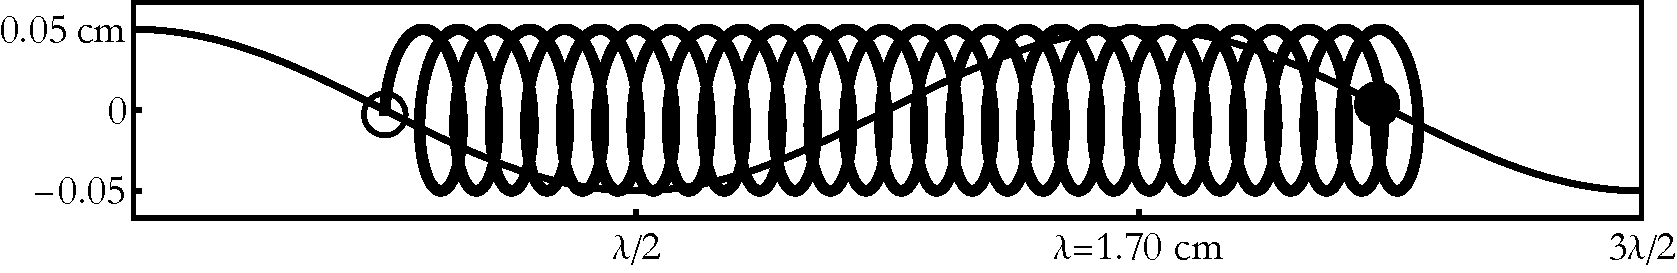
\includegraphics[width=1\linewidth]{Fig1a}}
	\caption{Траектории движения индивидуальных частиц нижней жидкости при докритических значениях тангенциального разрыва скоростей.}
	\label{ris:Fig1}
\end{figure}
Рассмотрим траектории движения жидких частиц для жидкостей с параметрами воды и воздуха при распространении по границе раздела синусоидальной волны с волновым числом, наиболее чувствительным по отношению к реализации неустойчивости Кельвина--Гельмгольца для этих жидкостей $ k=k_{cr} $.

На рисунке~\ref{ris:Fig1} демонстрируется траектория жидкой частицы нижней жидкости за 29 периодов волнового движения. Из~\eqref{Period} следует, что $ t_{\lambda}/T\perm=\zeta^{-2}k^{-2}\perm\approx 29.4 $ доля в периодах волнового движения, необходимая для дрейфа на расстояние соответствующее длине волны. Рисунок~\ref{ris:Fig1} останется неизменным при увеличении скорости $ U_{0} $  вплоть до критического значения  $ U_{cr}\approx 730\, \text{см/сек} $, при котором начинает развиваться неустойчивость Кельвина--Гельмгольца для рассматриваемых жидкостей, при измерении времени в долях волнового периода, а не в абсолютных значениях.

Рассуждая аналогичным образом можно внести поправку к лагранжевым компонентам скорости движения жидких частиц верхней жидкости. 

\begin{figure}[ht]
	\center{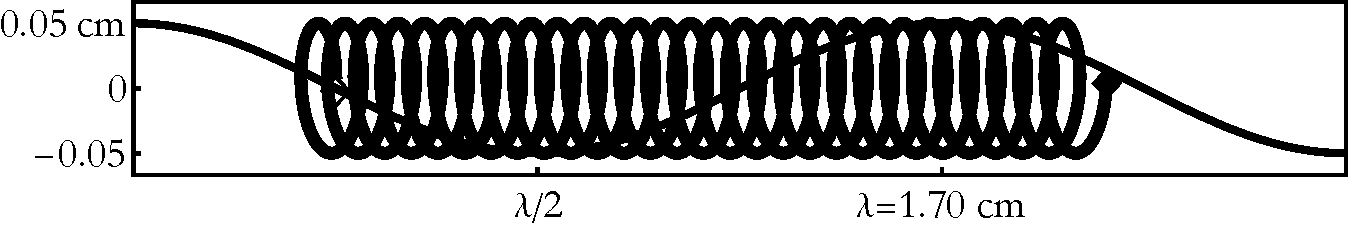
\includegraphics[width=1\linewidth]{Fig1b}}
	\caption{Траектории движения индивидуальных частиц верхней жидкости при значениях тангенциального разрыва скоростей меньше фазовой скорости волнового движения в системе отсчета, связанной с верхней жидкостью.}
	\label{ris:Fig2}
\end{figure}

На рисунке~\ref{ris:Fig2} построена траектория движения индивидуальных частиц верхней жидкости, движущейся со скоростью $ U_{0}=10\, \text{см/сек} $  в системе отсчета, связанной с верхней средой. 
Траектория построена за 53 периода волнового движения, поскольку именно такое время необходимо для дрейфа в движущейся вместе с верхней жидкостью системе отсчета. В неподвижной системе отсчета с учетом горизонтального сдвига $ U_{0} t' $ за время $ t'$  из~\eqref{Period'} следует, что доля, волновых периодов, необходимая для дрейфа жидкой частички на расстояние равное длине волны $ t'_{\lambda}/T=1/\left( \beta+\zeta^{2}k^{2}\left( 1-\beta \right) \right) \approx 2.2 $.
%Траектория построена за 2 периода волнового движения, поскольку из~\eqref{Period'} следует, что доля, волновых периодов, необходимая для дрейфа жидкой частички на расстояние равное длине волны $ t'_{\lambda}/T=1/\left( \beta+\zeta^{2}k^{2}\left( 1-\beta \right) \right) \approx 2.2 $. 
Траектории, аналогичные представленным на рисунке~\ref{ris:Fig2} будут наблюдаться у жидких частичек верхней жидкости при условии, когда скорость относительного сдвига не достигает фазовой скорости волнового движения $ 0<U_{0}<U_{ph} $.

Дальнейший рост $ U_{0} $ приводит к уменьшению модуля дрейфовой добавки и при достижении фазовой скорости $ U_{0}=U_{ph} $ добавка принимает нулевое значение, а период круговых движений жидкой частички стремится к бесконечному значению. Что соответствует равномерному и прямолинейному движению жидких частиц с фазовой скоростью волны $ U_{0}=U_{ph}\approx 23 \, \text{см/сек} $ (рисунок~\ref{ris:Fig3}). В системе отсчета движущейся в том же направлении со скоростью, равной фазовой скорости волнового движения поверхности, жидкие частицы верхней жидкости оказываются покоящимися.

\begin{figure}[ht]
	\center{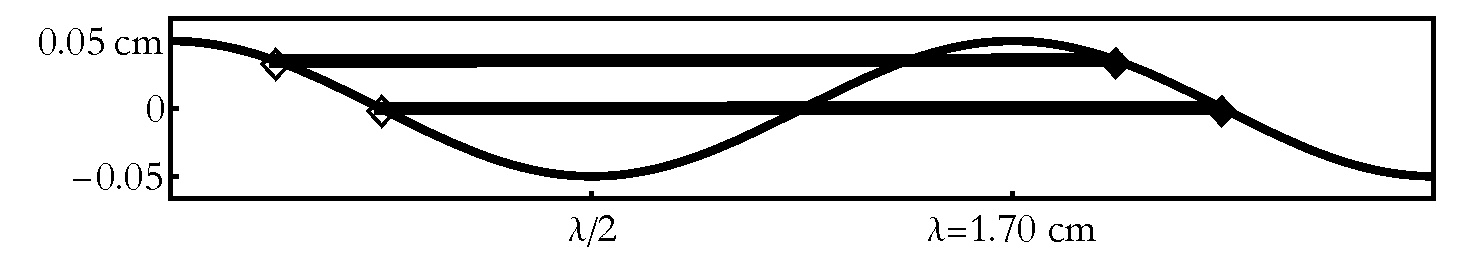
\includegraphics[width=1\linewidth]{Fig1c}}
	\caption{Траектории движения индивидуальных частиц верхней жидкости при значениях тангенциального разрыва скоростей равной фазовой скорости волнового движения.}
	\label{ris:Fig3}
\end{figure}

На рисунке~\ref{ris:Fig4} показана траектория движения жидкой частички из системы отсчета, движущейся вправо со скоростью относительного сдвига $ U_{0}=50\, \text{см/сек} $. При таком значении скорости $ U_{0} $ с учетом горизонтального сдвига $ U_{0} t' $ доля периода волнового движения необходимая для дрейфа на расстояние равное длине волны  $ t'_{\lambda}/T=1/\left( \beta+\zeta^{2}k^{2}\left( 1-\beta \right) \right) \approx 0.5 $. В движущейся системе отсчета для дрейфа на расстояние длины волны необходимо около 27 периодов волнового движения (именно за это время построена траектория движения на рисунке~\ref{ris:Fig4}).  Подобная картина будет наблюдаться для всех значений скорости $ U_{0} $ при выполнении неравенства $ U_{ph}<U_{0}<U_{cr} $.

\begin{figure}[ht]
	\center{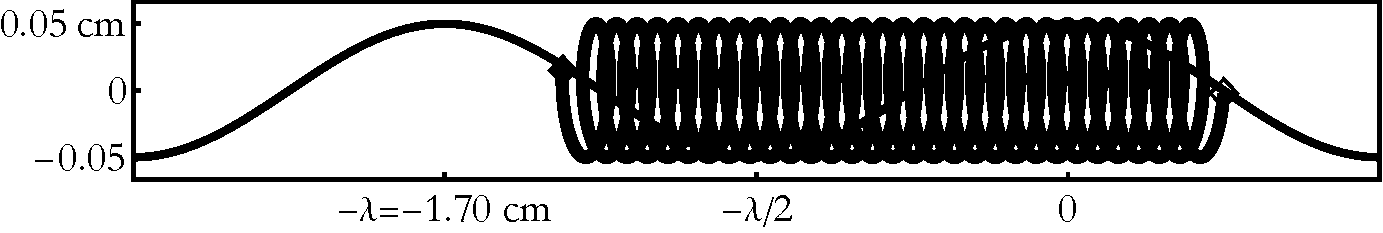
\includegraphics[width=1\linewidth]{Fig1d}}
	\caption{Траектории движения индивидуальных частиц верхней жидкости при значениях тангенциального разрыва скоростей больше фазовой скорости волнового движения в системе отсчета, связанной с верхней жидкостью.}
	\label{ris:Fig4}
\end{figure}

Материальные частицы, составляющие верхнюю и нижнюю жидкости участвуют в дрейфовых и циклических движениях. В круговых движениях лидирующими являются слагаемые первого по амплитуде порядка малости, а в дрейфовых компонентах скорости наиболее значимой оказываются добавки второго порядка малости, пропорциональные квадрату амплитуды $ \zeta^{2} $. В работе производится учет обоих типов движения, сохраняя только главные члены асимптотического разложения.

В рассматриваемой системе жидкостей граница раздела способна дестабилизироваться в виде неустойчивости Кельвина--Гельмгольца. В присутствии поверхностного натяжения на границе раздела, характеризуемого коэффициентом поверхностного натяжения $ \gamma $ и ускорения свободного падения $ g $ неустойчивость носит пороговый характер  и развивается, если скорость относительного движения превышает некоторое критическое значение $ U_{cr} $.

Мнимая составляющая $ r=Im\left(\omega\right) $ принимает положительные значения для одного из корней дисперсионного уравнения и отрицательные для другого. Значение $ r>0 $  характеризует инкремент нарастания неустойчивости Кельвина--Гельмгольца, связанной с волновым возмущением границы раздела с волновым числом $ k $. Корень с таким значением параметра $ r $ представляет интерес для рассмотрения в настоящей работе.

На начальном этапе развития неустойчивости поле скоростей модифицируется: появляется дополнительный множитель, экспоненциально нарастающий со временем $ \propto \exp \left( r t\right) $. То же самое касается и скорости дрейфа в нижней жидкости и дрейфовой добавки в верхней. При этом дрейфовые добавки оказываются направлены в противоположные стороны и их экспоненциальный рост со временем должен приводить к уменьшению тангенциального разрыва скоростей, и как следствие, к стабилизации поверхности.

\underline{\textbf{Третья глава}} посвящена обобщению разработанной методики с учетом факторов оказывающих влияние на круговую частоту волнового движения (на примере поверхностного электрического заряда) и на модуляцию амплитуды волнового движения (на примере волнового возмущения в виде простейшего волнового пакета Стокса), также рассмотрено применение методики с учетом совместного влияния этих двух факторов. 

Рассматривается случай, когда волновое возмущение представляет из себя не простейшую синусоидальную волну, а сформировано волновым пакетом Стокса, состоящего из двух капиллярно--гравитационных волн одинаковой амплитуды  $ \zeta $ с волновыми числами  $ k_{\pm}=k \pm \Delta k $, отличающимися друг от друга на малую величину  $ 2 \Delta k \ll k $. Значение $ k $  характеризует волновое число несущей волны, а  $ \Delta k $~--- волновое число огибающей волнового пакета. Круговые частоты волн, составляющих пакет $ \omega_{\pm} $ определяются из дисперсионного уравнения:
\begin{equation}
\omega_{\pm}=\omega \pm \Delta \omega = \sqrt{g k _{\pm} \left( 1+ k_{\pm}^{2} \alpha^{2} \right)}
\label{DispUrPack}
\end{equation}

Здесь стоит отметить, что в дисперсионное уравнение~\eqref{DispUrPack} неявным образом (в составе волновых чисел $ k_{\pm} $ ) входит параметр $ \Delta k $, считающийся малым, а символ $ \alpha= \sqrt{\gamma/\rho g} $  обозначает капиллярную постоянную жидкости. 

Выражение для отклонения границы раздела $ \xi_{1} $ от равновесного положения принимает вид:
\begin{equation}
\xi_{1}=2\zeta \cos \left( \omega t - k x \right) \cos \left( \Delta \omega t - \Delta k x \right)
\label{WavePacket}  
\end{equation}

Из соотношения~\eqref{WavePacket} естественным образом выделяется два временных масштаба $ T=2\pi/\omega $~--- период несущей волнового пакета, характеризующий быстрые изменения во времени и $ \tau=2\pi/\Delta \omega $~--- период огибающей, характеризующий медленно меняющиеся процессы. 

%Произведем расчет скорости дрейфа, следуя разработанной методике и выделяя медленно меняющиеся со временем слагаемые. В явном виде дрейфовая скорость $ D $ выглядит следующим образом:
%\begin{gather}
%\begin{gathered}
%D=\zeta^{2} \left[ \left( k \omega +\Delta k \left( k V_{g}+\omega \right) \right) \exp \left( 2 k_{+}z \right) + \right.\\
%+\left( k \omega - \Delta k \left( k V_{g}+\omega \right) \right) \exp \left( 2 k_{-}z \right)+\\
%+2 k \omega \cos \left( 2 t V_{g} \Delta k - 2 x \Delta k \right) \exp \left( 2 k z \right) +\\
%\left. +2 \omega \Delta k \cos \left( 2 t V_{g} \Delta k - 2 x \Delta k \right) \exp \left( 2 \Delta k z \right) \right]
%\label{DriftPack}
%\end{gathered}
%\end{gather}
%
%Важно отметить, что расчет дрейфовой скорости  произведен в линейном приближении по отклонению волновых чисел волн в пакете друг от друга  $ \Delta k $. Слагаемые, пропорциональные $ \Delta k $  в более высоких степенях отбрасывались в силу малости и громоздкости. Такое приближение должно удовлетворить большинство расчетных задач, однако при помощи представленной методики можно воспроизвести дрейфовую скорость целиком. Стоит пояснить смысл произведенной замены  $ \Delta \omega \rightarrow V_{g} \Delta k $. В дисперсионное уравнение входит небольшая добавка к волновому числу  $ \Delta k $, считая ее малой и разлагая частоту волнового движения в ряд Маклорена, в линейном приближении получим:
%\begin{equation*}
%\omega_{\pm}=\omega \pm \Delta \omega = \omega \pm \partial_{k} \omega \Delta k.
%\end{equation*}
%
%Причем частная производная  $ \partial_{k}\omega = V_{g} $ играет роль групповой скорости волнового пакета.

%Сравним скорость дрейфового движения  со скоростью классического дрейфа Стокса~\eqref{UdriftNizh}. Первое отличие, бросающееся в глаза~--- зависимость скорости дрейфа  от времени, которое должно наблюдаться на небольших интервалах времени в эксперименте (время наблюдения $ t_{obs} $  должно быть сравнимо с периодом несущей волнового пакета $ T $). Если же время наблюдения велико (по сравнению с периодом огибающей волнового пакета $ t_{obs}\gg T $ ), то имеет смысл говорить об усредненной скорости дрейфового движения за период огибающей волнового пакета  $ \left\langle D \right\rangle   $:
%\begin{gather}
%\begin{gathered}
%\left\langle D\right\rangle  = \zeta^{2}\left[ \left( k \omega + \Delta k \left( k V_{g} + \omega \right) \right) \exp \left( 2 k_{+} z \right) + \right. \\
%\left. + \left( k \omega - \Delta k \left( k V_{g} + \omega \right) \right) \exp \left( 2 k_{-} z \right) \right]
%\label{SRDrift}
%\end{gathered}
%\end{gather}
Были получены выражения для дрейфовых скоростей в линейном приближении по отклонению волновых чисел волн в пакете друг от друга  $ \Delta k $. Слагаемые, пропорциональные $ \Delta k $  в более высоких степенях отбрасывались в силу малости и громоздкости. Такое приближение должно удовлетворить большинство расчетных задач, однако при помощи представленной методики можно воспроизвести дрейфовую скорость целиком. Сравнение полученных дрейфовых скоростей со скоростью классического дрейфа Стокса~\eqref{UdriftNizh} выявило следующее принципиальное отличие: зависимость скорости дрейфа  от времени, которое должно наблюдаться на небольших интервалах времени в эксперименте (время наблюдения $ t_{obs} $  должно быть сравнимо с периодом несущей волнового пакета $ T $). Если же время наблюдения велико (по сравнению с периодом огибающей волнового пакета $ t_{obs}\gg T $ ), то имеет смысл говорить об усредненной скорости дрейфового движения за период огибающей волнового пакета.
Расчеты показывают, что усредненная за период огибающей волнового пакета скорость дрейфа  принимает значения примерно в два раза меньшие, чем скорость классического дрейфа Стокса. Такая же тенденция должна сохраняться для произвольного цуга волн. Таким образом в эксперименте дрейф Стокса нужно ожидать в разы меньшим, чем это предсказывает классическая теория Стокса.

Поверхностный электрический заряд, как и тангенциальный разрыв скоростей является фактором, дестабилизирующим поверхность и оказывающим влияние на круговую частоту волнового движения. При достижении поверхностным электрическим зарядом некоторого критического значения поверхность жидкости дестабилизируется и волновое возмущение принимает апериодический характер. На поверхности при этом образуются конусообразные выступы, называемые «конусы Тейлора», с вершин которых сбрасывается излишек электрического заряда в виде маленьких сильнозаряженных капель жидкости. Явление неустойчивости поверхности жидкости по отношению к избытку поверхностного электрического заряда получило название «неустойчивость Тонкса--Френкеля». Это явление используется при электродиспергировании различных жидкостей, например, лакокрасочных материалов; получении жидкометаллических ионов; а также связано с теорией атмосферного электричества. В основном интерес для исследователей представляло поведение жидкости при закритических значениях электрического заряда. Закономерности поведения волнового возмущения жидкости при докритических значениях плотности поверхностного электрического заряда в настоящий момент изучены слабо, однако докритический поверхностный электрический заряд может играть роль регулятора скорости дрейфа Стокса. Это связано с тем, что электрический заряд в качестве параметра входит в дисперсионное уравнение, определяющее связь волнового числа с круговой частотой и, как следствие, оказывает влияние на фазовую скорость волнового движения, инициирующего дрейф Стокса. Дисперсионное уравнение для капиллярно-гравитационных волн, распространяющихся вдоль свобдной электрически заряженной с поверхностной плотностью $ \kappa_{0} $ поверхности идеальной жидкости описывается соотношением:
\begin{equation}
\omega = \sqrt{gk \left( 1+k^{2}\alpha^{2}-k\alpha W \right)}; \qquad \qquad  W=\dfrac{4 \pi \kappa_{0}^{2}}{\sqrt{\rho g \gamma}}.
\label{DUTF}
\end{equation}

Здесь $ W $~--- безразмерный параметр, характеризующий отношение электрических и лапласовских сил на поверхности жидкости, имеющий название параметр Тонкса--Френкеля. Его физический смысл~--- безразмерная поверхностная плотность электрического заряда.

Анализ дисперсионного уравнения показал, что круговая частота капиллярно-гравитационных волн уменьшается с увеличением поверхностного электрического заряда и принимает нулевое значение при критическом значении параметра Тонкса--Френкеля $ W_{*}=\alpha k +1/\alpha k  $. Критическое значение поверхностного электрического заряда соответствует прекращению круговых движений жидких частиц и, следовательно, дрейфа.

\begin{figure}[ht]
	\begin{minipage}[h]{0.47\linewidth}
		\center{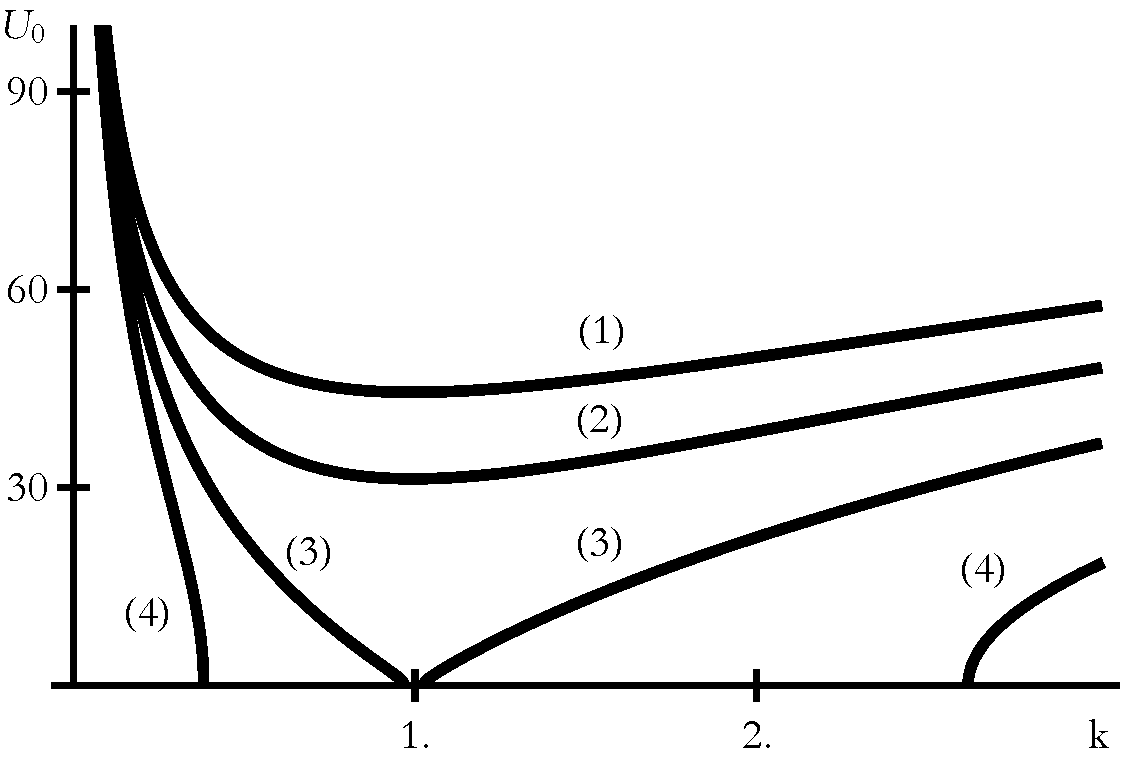
\includegraphics[width=1\linewidth]{Fig2a}} \\а) \\
	\end{minipage}
	\hfill
	\begin{minipage}[h]{0.47\linewidth}
		\center{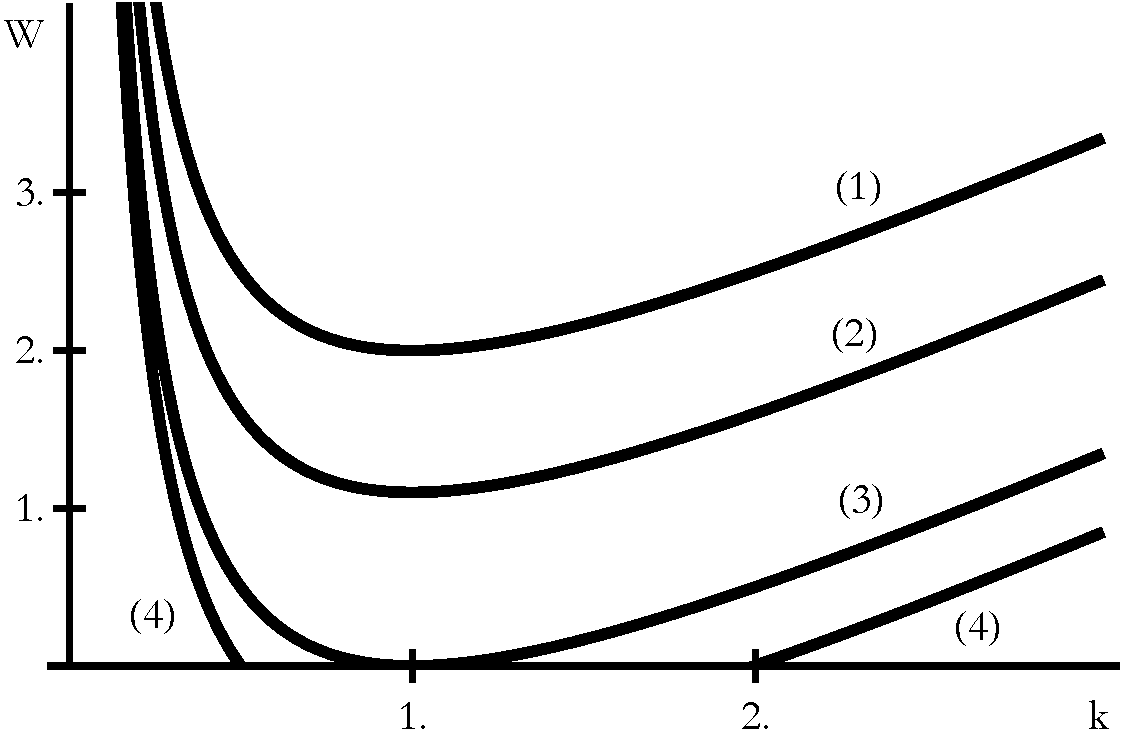
\includegraphics[width=1\linewidth]{Fig2b}} \\б)
	\end{minipage}
	\label{ris:Fig5}
		\caption{Кривая нейтральной устойчивости в области параметров а)~$ \left(U_{0}, k	\right) $ б)~$ \left(W, k	\right) $.}
\end{figure}

Анализ задачи, в которой учтены все перечисленные выше факторы показал, что поверхностный электрический заряд и тангенциальный разрыв скоростей на границе раздела усиливают дестабилизирующие свойства друг друга. На рисунке~\ref{ris:Fig5}~(а) представлены кривые нейтральной устойчивости в безразмерных переменных $ \rho=g=\gamma=1 $ в области параметров $ \left(U_{0}, k	\right) $ для разных значений поверхностного электрического заряда. Кривой~(1) соотвествует значение параметра Тонкса--Френкеля $ W=0 $, кривой (2)~--- $ W=1 $, кривой (3)~--- $ W=2 $, кривой (4)~--- $ W=3 $. На рисунке~\ref{ris:Fig5}~(б) представлены кривые нейтральной устойчивости в области безразмерных параметров $ \left(W, k	\right) $ для разных значений тангенциального разрыва скоростей. Кривой~(1) соотвествует значение тангенциального разрыва скоростей $ U_{0}=0 $, кривой (2)~--- $ U_{0}=30 $, кривой (3)~--- $ U_{0}=44.7 $, кривой (4)~--- $ U_{0}=50 $. Таким образом в присутствии электрического заряда на границе раздела жидкостей совместная неустойчивость Кельвина--Гельмгольца и Тонкса--Френкеля реализуется при меньших значениях тангенциального разрыва скоростей и наоборот: в присутствии относительного движения необходим меньший электрический заряд для перехода границы раздела жидкостей в неустойчивое состояние.  

В \underline{\textbf{четвертой главе}} рассматривается вязкая жидкость с кинематической вязкостью $ \nu $, по поверхности которой равномерно с поверхностной плотностью $ \Gamma_{0} $ распределено поверхностно-активное вещество (ПАВ), образующее нерастворимую плёнку. Необходимо учесть, что в процессе распространения волны на деформированной волновым движением поверхности жидкости будет происходить перераспределение ПАВ, и следовательно поверхностную плотность ПАВ следует считать функцией времени и горизонтальной координаты $ \Gamma=\Gamma \left( t, x \right) $. Локальные изменения поверхностной плотности ПАВ вызывают локальные изменения величины коэффициента поверхностного натяжения $ \gamma $. Принималось, что плёнка ПАВ и верхний слой жидкости находятся в термодинамическом равновесии, поэтому изменение локального значения поверхностной плотности ПАВ мгновенно вызывает изменение локального значения коэффициента поверхностного натяжения в соответствии с изотермой $ \gamma = \gamma \left( \Gamma \right) $, считающейся известной. Получено дисперсионное уравнение для комплексной частоты волнового движения $ S\equiv r+i\omega $:
\begin{equation}
\left( \left( \Omega +2N \right)^{2} +1-\dfrac{L}{\Omega^{2}} \right) \left( 1-L \dfrac{1+\Omega^{2}}{4 \Omega^{2} N^{2}}\right)^{-1}=4N^{3/2} \sqrt{\Omega +N};
\label{DispUrPAV}
\end{equation}
\begin{equation*}
\Omega \equiv \dfrac{S}{\omega_{0}}; \qquad N \equiv \dfrac{\nu k^{2}}{\omega_{0}}; \qquad L \equiv \dfrac{\Pi k^{3}}{\rho \omega_{0}^{2}}; \qquad \omega_{0}^{2}=k g \left( 1+\dfrac{\gamma_{0}}{\rho g}k^{2}\right);
\end{equation*}
\begin{equation*}
\gamma_{0} \equiv \gamma \left( \Gamma_{0} \right);\qquad \gamma_{\Gamma} \equiv \left(\dfrac{d \gamma}{d \Gamma} \right)_{0}; \qquad \Pi = \gamma_{\Gamma} \Gamma_{0}.
\end{equation*}
 Значение $ \gamma_{\Gamma} $ характеризует наклон касательной к кривой, изображающей зависимость $ \gamma = \gamma \left( \Gamma \right) $ и для обычных ПАВ, уменьшающих поверхностное натяжение, принимает отрицательные значения $ \gamma_{\Gamma}<0 $. Параметр $ \Pi $ называют упругостью плёнки. Он имеет размерность силы на единицу длины и характеризует упругие свойства плёнки ПАВ и также как $ \gamma_{\Gamma} $ для обычных ПАВ, принимает отрицательные значения. Изменение модуля $ \Pi $ для определенного ПАВ можно осуществить изменяя среднее значение концентрации $ \Gamma_{0} $: при нулевой средней концентрации $ \Pi=0 $ и $ \vert \Pi \vert $ растет с ростом средней концентрации $ \Gamma_{0} $. Использованный здесь вспомогательный параметр $ \omega_{0} $ имеет смысл круговой частоты волнового движения на поверхности бесконечно глубокой идеальной жидкости с капиллярной постоянной, равной $ \sqrt{\gamma_{0}/\left( \rho g \right)} $. Безразмерный параметр $ N $ характеризует роль вязкости при волновом движении. Если $ N\ll 1 $, то жидкость принято считать маловязкой.

Анализ дисперсионного уравнения~\eqref{DispUrPAV} показал, что в присутствии ПАВ на поверхности жидкости реализуется два типа волновых движений: капиллярно-гравитационные волны и волны Марангони, инициируемые касательными натяжениями, возникающими в упругой плёнке при распространении волн сжатий и растяжений. Было обнаружено, что при некотором характерном значении упругости плёнки ПАВ (своём для каждого волнового числа) круговые частоты капиллярно-гравитационных волн и волн Марангони сравниваются. При этом характерном значении декремент затухания капиллярно-гравитационных волн принимает своё максимальное значение. При достижении максимального эффекта гашения волн (достижения модулем упругости пленки ПАВ характерного значения максимум концентрации ПАВ располагается на середине среза волны. с уменьшением упругости пленки максимум оказывается ближе к вершине горба волнового возмущения поверхности жидкости. Увеличение упругости приводит к смещению максимума концентрации ближе ко впадине волнового возмущения. Эти особенности демонстрируются на рисунке~\ref{ris:Fig7} в безразмерных переменных $ \rho=g=\gamma_{0}=1 $ для жидкости с безразмерной вязкостью $ \nu=0.002 $, что соответствует жидкости с параметрами воды. 

\begin{figure}[ht]
	\begin{minipage}[h]{0.47\linewidth}
		\center{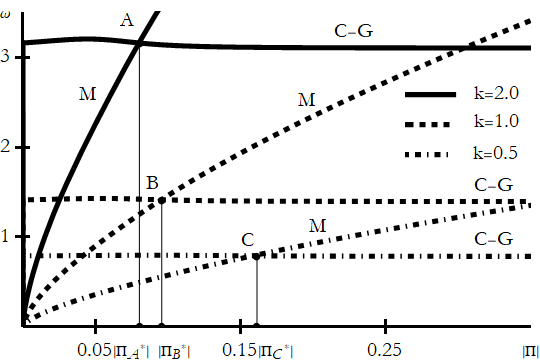
\includegraphics[width=1\linewidth]{Fig3a}} а) \\
	\end{minipage}
	\hfill
	\begin{minipage}[h]{0.47\linewidth}
		\center{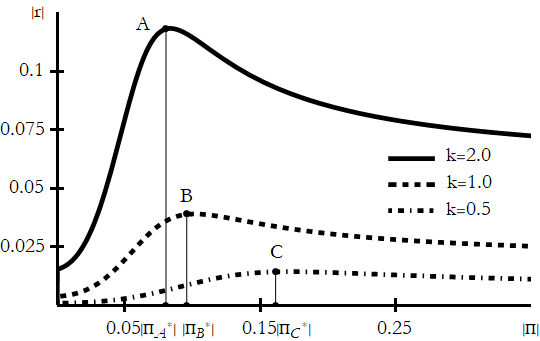
\includegraphics[width=1\linewidth]{Fig3b}} \\б)
	\end{minipage}
	\vfill
		\center{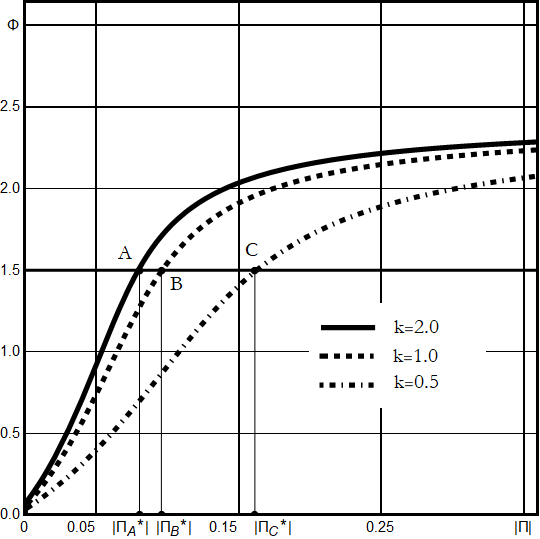
\includegraphics[width=0.47\linewidth]{Fig3c}} \\в) \\
	\caption{Зависимость от упругости пленки для разных длин волн а)~круговых частот $ \omega $ капиллярно-гравитационных волн и волн Марангони б)~декрементов затухания $ |r| $ капиллярно-гравитационных волн в)~разности фаз $ \Phi $ между положением максимума концентрации ПАВ и гребнем волны.}
	\label{ris:Fig7}
\end{figure}

Было исследовано влияние ПАВ на траектории движения индивидуальных жидких частиц. Анализ показал, что в отсутствии ПАВ жидкие частицы в линейном приближении по амплитуде волны движутся практически по окружностям. С увеличением упругости круговые траектории «сплющиваются» в эллипсы и при достижении характерного значения упругости вырождаются в отрезки прямых. Дальнейший рост упругости пленки приводит к «выворачиванию» траекторий: жидкие частицы снова движутся по эллипсам, но при этом изменяют направление обхода внутренней части траектории на противоположное. В качестве примера рассмотрены траектории движения индивидуальных частиц жидкости с параметрами воды в безразмерных переменных, вызванного распространением волны с безразмерным волновым числом $ k=1 $ (см. рисунок~\ref{ris:Fig8}).

\begin{figure}[ht]
	\center{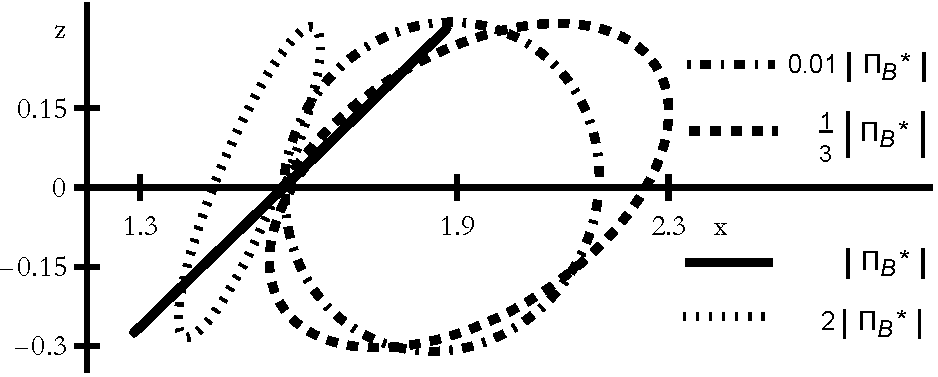
\includegraphics[width=0.7\linewidth]{Fig4}}
	\caption{Траектории движения индивидуальной жидкой частицы в зависимости от упругости плёнки ПАВ.}
	\label{ris:Fig8}
\end{figure}

Было исследовано влияние тангенциального разрыва скоростей на динамику волнового движения в присутствии ПАВ и на характер перераспределения ПАВ вдоль границы раздела в модели, в которой нижняя жидкость вязкая и покрыта упругой нерастворимой плёнкой ПАВ, а верхняя~--- идеальная, движущаяся относительно нижней с постоянной горизонтальной скоростью. На примере волны с безразмерным волновым числом  $ k=1 $ показано, что скорость движения верхней среды (при  докритических значениях с точки зрения неустойчивости Кельвина--Гельмгольца) практически не изменяет круговую частоту волн Марангони и заметно уменьшает круговую частоту капиллярно--гравитационных волн (см. рисунок~\ref{ris:Fig9}~а). Максимальное значение декремента затухания капиллярно--гравитационных волн при этом уменьшается и сдвигается в область меньших значений упругости плёнки ПАВ (см. рисунок~\ref{ris:Fig9}~б). Положение максимума концентрации ПАВ также достигает середины склона, следующего за горбом в направлении распространения волны при достижении максимального эффекта гашения капиллярно--гравитационных волн. (см. рисунок~\ref{ris:Fig9}~в).

\begin{figure}[ht]
	\begin{minipage}[h]{0.47\linewidth}
		\center{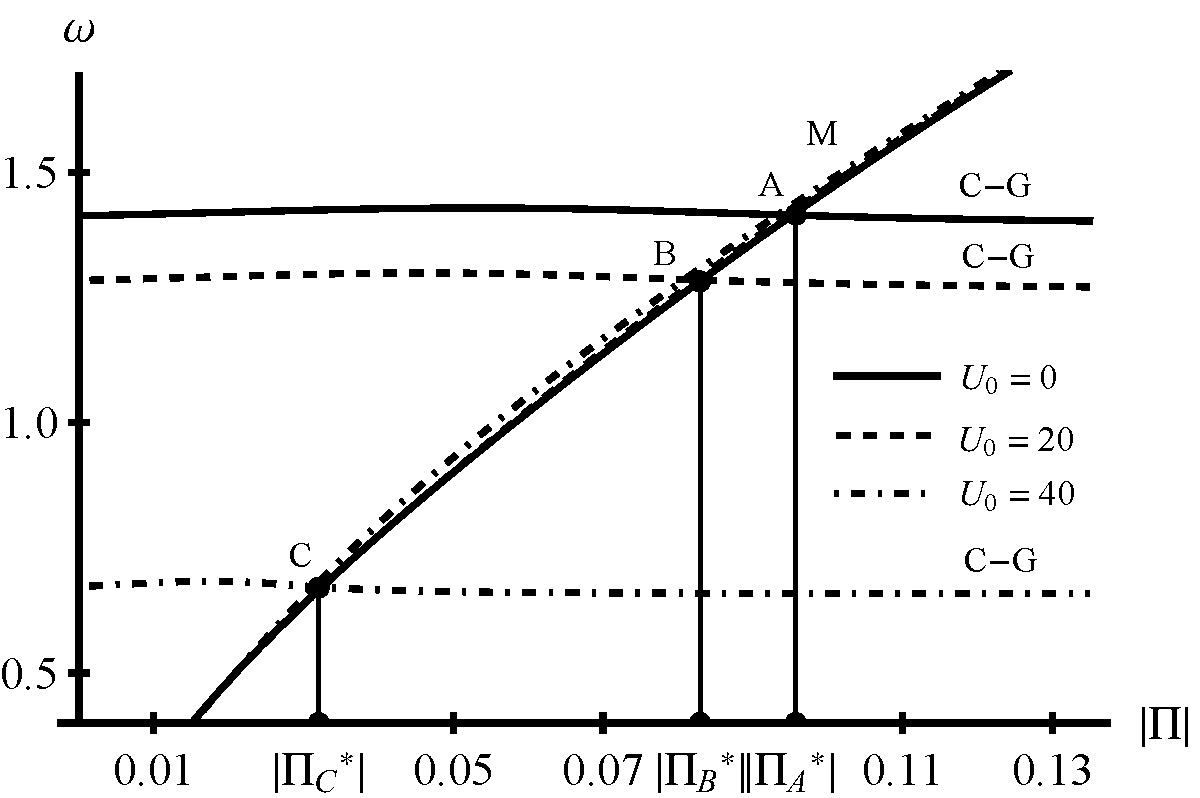
\includegraphics[width=1\linewidth]{Fig5a}} а) \\
	\end{minipage}
	\hfill
	\begin{minipage}[h]{0.47\linewidth}
		\center{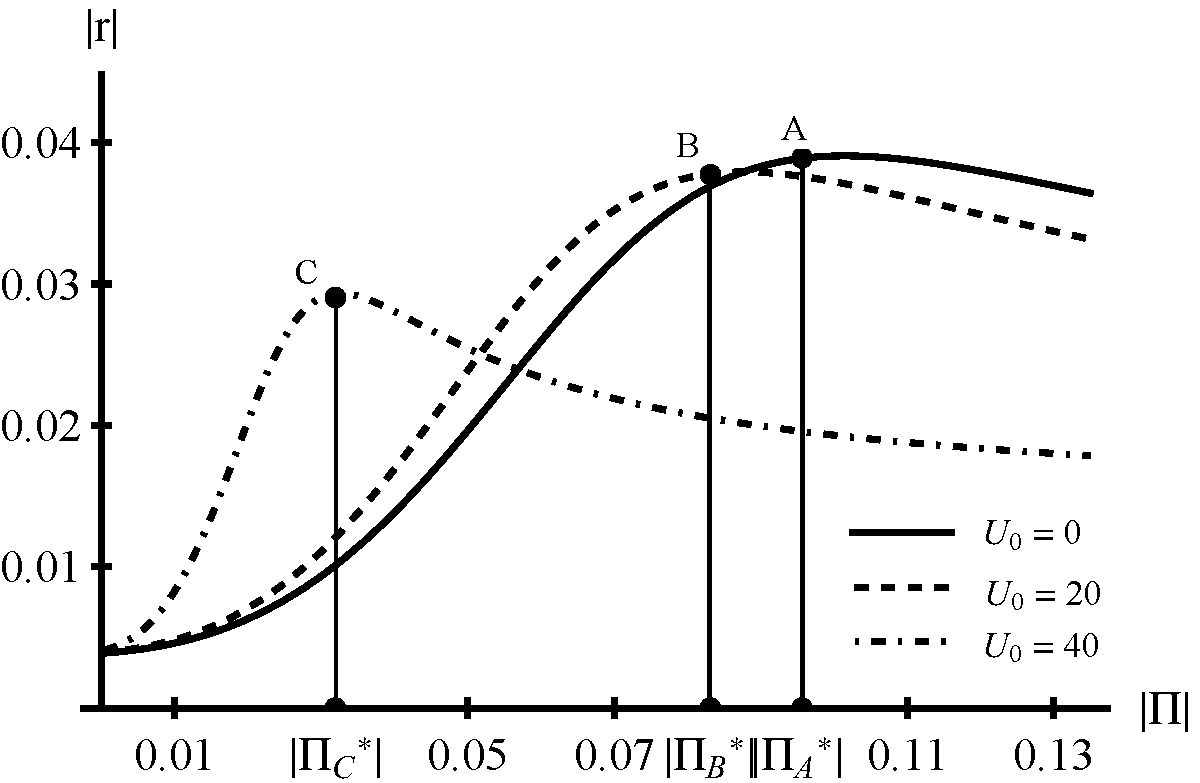
\includegraphics[width=1\linewidth]{Fig5b}} \\б)
	\end{minipage}
	\vfill
	\center{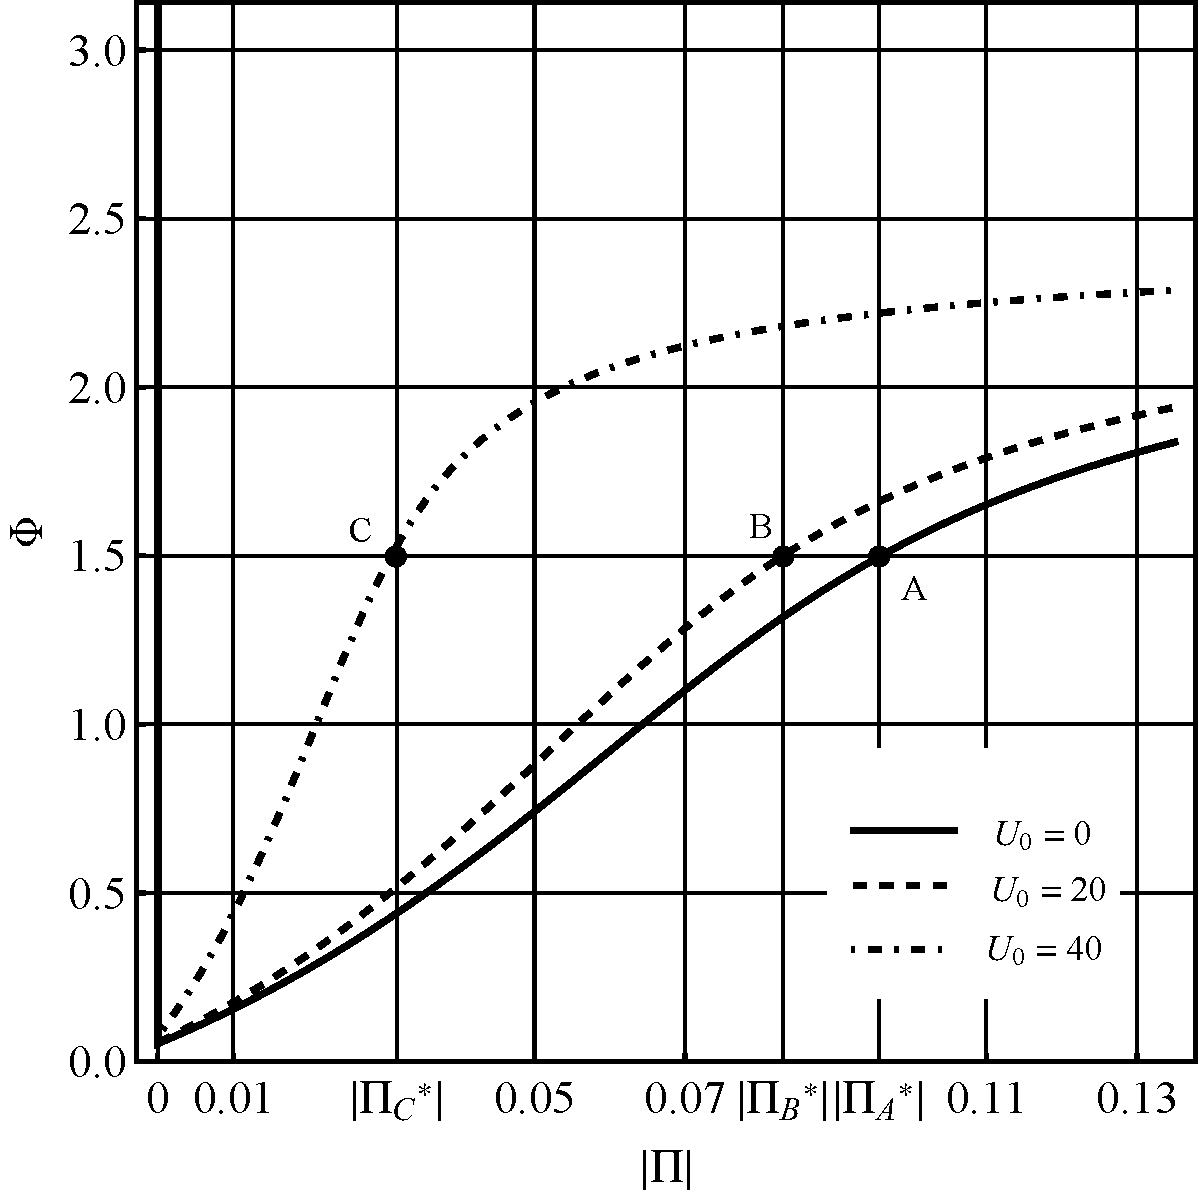
\includegraphics[width=0.47\linewidth]{Fig5c}} \\в) \\
	\caption{Зависимость от упругости пленки для волны с безразмерным волновым числом $ k=1 $ при разных значениях безразмерного тангенциального разрыва скоростей а)~круговых частот $ \omega $ капиллярно-гравитационных волн и волн Марангони б)~декрементов затухания $ |r| $ капиллярно-гравитационных волн в)~разности фаз $ \Phi $ между положением максимума концентрации ПАВ и гребнем волны.}
	\label{ris:Fig9}
\end{figure}

Были исследованы скорости дрейфовых движений, инициированных распространением волны вдоль поверхности жидкости. Было получено выражение для скорости дрейфа

\begin{equation}
U_{drift}=w_{d}+u_{b}+u_{c};
\label{UdriftPAV}
\end{equation}
\vspace{-15pt}
\begin{multline}
w_{d}= \zeta^{2} \dfrac{\exp \left( 2 r t \right)}{2 \vert S \vert^{2}}\left( 2 \vert A \vert^{2} k \omega \exp \left( 2 k z \right)+ M_{0} \exp \left( 2 \beta z \right) +\right.\\
\left.+\left( M_{1}\cos \left( \eta z \right) +M_{2} \sin \left( \eta z \right) \right) \exp \left( \left( k+\beta \right) z \right) \right)
\label{wdPAV}
\end{multline}
\noindent
\begin{gather*}
M_{0}= k \vert B \vert^{2} Im \left( \left( \dfrac{q}{q^{*}}+1 \right) S \right);\\
M_{1}=Im \left( A^{*} B \left( q S - \dfrac{k^{2}}{q}S^{*} \right) \right)+2 Re \left( A B^{*} \right) k \omega;\\
M_{2}=Re\left( A^{*} B \left( q S - \dfrac{k^{2}}{q}S^{*} \right) \right) + 2 Im \left( A B^{*} \right) k \omega.
\end{gather*}

Компонента $ u_{b} $ вычисляется по  формуле:
\begin{multline}
u_{b} \equiv u_{b} \left( z, t \right) = \zeta^{2}  i k \dfrac{\vert B \vert^{2} \left( q^{2}-q^{*2}\right)}{4 \vert q \vert^{2} \left( 2 r-\nu \left( q + q^{*} \right)^{2}\right)} \exp \left( 2 r t+ \left( q+q^{*}\right) z \right)+ \\
+\zeta^{2} \left( \dfrac{i A^{*} B \left( q^{2} - k^{2} \right)}{4 q \left( 2 r - \nu \left( q+k \right)^{2} \right)} \exp \left( 2 r t +\left( q+k\right) z \right) +C.C. \right),
\label{Ub}
\end{multline}
а слагаемое $ u_{c} $ определяется выражениями:
\begin{multline}
u_{c} \equiv u_{c} \left( z, t \right) = \zeta^{2} \Lambda \left( \sqrt{\dfrac{\nu}{\pi}} \int_{0}^{t} \exp \left( - \dfrac{z^{2}}{4 \nu \left( t - \eta \right)} \right) \dfrac{\exp \left( 2 r \eta \right)}{\sqrt{t - \eta}}d \eta +\right.\\
\left. + \sqrt{\dfrac{1}{\pi \nu t}} \int_{0}^{\infty} \left( \exp \left( -\dfrac{\left( z - \sigma \right)^{2}}{4 \nu t} \right) + \exp \left( -\dfrac{\left( z + \sigma \right)^{2}}{4 \nu t} \right) \right) \Psi \left( \sigma \right) d \sigma\right);
\label{UcYavVid}
\end{multline}
\begin{equation*}
\Psi \left( z \right) \equiv u_{c}\left( 0, z \right); \qquad q=\sqrt{k^{2}+\dfrac{S}{\nu}};
\end{equation*}
\begin{gather*}
A=i S \left( \dfrac{q}{k - q} + \dfrac{\rho \nu k S}{\rho \nu \left( k+q \right) S - k^{2} \Pi}\right); \qquad B=\dfrac{i k q S \left( 2\rho \nu S - k \Pi \right)}{\left( q-k \right) \left( \rho \nu \left( k+q \right) S - k^{2} \Pi \right)}.
\end{gather*}

Показано, что в сумме слагаемые $ u_{b} + w_{d} $ экспоненциальным образом зависят от глубины и в пределе малой вязкости с точностью до множителя, учитывающего вязкую диссипацию, совпадает с классической формулой для скорости дрейфа Стокса и переходит в эту формулу при $ \nu=0 $. Принципиально, что не отдельные слагаемые, а именно их сумма $ w_{d}+u_{b} $ реализует асимптотическое соответствие между моделями дрейфа в вязкой и в идеальной жидкости. При произвольной вязкости скорость суммарного течения $ w_{d}+u_{b} $ сохраняет экспоненциальный характер зависимости от своих аргументов. Компонента $ u_{c} $ среднего течения~\eqref{UdriftPAV} не экспоненциальным, а более сложным образом зависит от своих аргументов~\eqref{UcYavVid} и отвечает за «добавочное течение», возникающее благодаря средним горизонтальным вязким напряжениями, действующим между горизонтальными слоями жидкости, двигающимися в среднем с разными скоростями.


В \underline{\textbf{заключении}} приведены основные результаты работы, которые заключаются в следующем:
%% Согласно ГОСТ Р 7.0.11-2011:
%% 5.3.3 В заключении диссертации излагают итоги выполненного исследования, рекомендации, перспективы дальнейшей разработки темы.
%% 9.2.3 В заключении автореферата диссертации излагают итоги данного исследования, рекомендации и перспективы дальнейшей разработки темы.
\begin{enumerate}
	\item Разработана аналитическая асимптотическая методика перехода от описания поля скоростей в переменных Эйлера к описанию в переменных Лагранжа. Методика позволяет совершать аналитический асимптотический переход с учетом горизонтальных сдвиговых движений жидкостей.
	\item Обнаружено свойство неустойчивости Кельвина--Гельмгольца, заключающееся в формировании дрейфовых течений в контактирующих жидкостях, направленных таким образом, чтобы скомпенсировать тангенциальный разрыв скоростей, инициировавший неустойчивость.
	\item Аналитически получены результаты расчета влияния поверхностного электрического заряда на скорость дрейфа и траектории движения индивидуальных частиц жидкости, связанные с распространением по поверхности жидкости капиллярно--гравитационной волны. Поверхностный электрический заряд уменьшает скорость дрейфовых движений, за счет уменьшения круговой частоты волнового движения (увеличения эйлерова периода) и увеличивает лагранжев период волнового движения (уменьшает частоту обращения индивидуальной частицы жидкости вокруг среднего положения). 
	\item Аналитически определено влияние амплитудной модуляции капиллярно--гравитационного волнового возмущения поверхности жидкости, на скорость инициируемого дрейфа и траектории движения индивидуальных частиц жидкости. При распространении волнового пакета вдоль поверхности жидкости средние дрейфовые течения оказываются примерно в двое меньшими по сравнению с течениями, связанными с распространением простейшей синусоидальной волны. 
	\item Аналитически установлено влияние плёнки поверхностно--активного вещества на траектории движения индивидуальных частиц жидкости. С увеличением упругости плёнки ПАВ уменьшается внутренняя площадь траектории, заметаемой индивидуальной жидкой частицей за период. При достижении упругостью плёнки ПАВ характерного значения, траектории вырождаются в отрезки прямых, наклоненных к горизонту под углом около $ \pi/4 $. Дальнейший рост упругости приводит к возникновению круговых движений с изменением направления обхода траектории.
	\item Разработано аналитическое представление о перераспределении поверхностно--активного вещества, связанного с распространением капиллярно--гравитационной волны по поверхности вязкой жидкости. Предложенные формулы позволяют проследить за положением максимума концентрации плёнки ПАВ, покрывающей вязкую жидкость в зависимости от упругости и связать это распределение с декрементами затухания капиллярно--гравитационных волн, распространяющихся вдоль поверхности жидкости.
	\item Аналитически определены скорости дрейфового течения, инициируемого волновым движением вдоль поверхности вязкой жидкости, покрытой плёнкой поверхностно--активного вещества. Выделены составляющие дрейфового движения, затухание которых с глубиной носит экспоненциальный характер и являющиеся преемственными классическому дрейфу Стокса и составляющие, связанные с наличием упругих напряжений между слоями вязкой жидкости. Определено влияние ПАВ на эти компоненты скорости дрейфа.
	
	
%  \item Разработана аналитическая асимптотическая методика расчета траекторий движения индивидуальных жидких частиц, участвующих в циклическом и дрейфовом движениях, связанных с распространением волны или волнового пакета Стокса вдоль поверхности жидкости.
%  \item Обнаружено новое свойство неустойчивости Кельвина--Гельмгольца, заключающееся в формировании дрейфовых течений в контактирующих жидкостях, направленных таким образом, чтобы уменьшить тангенциальный разрыв скоростей, инициировавший развитие неустойчивости.
%  \item Обнаружено значение упругости пленки ПАВ, при котором затухание волнового движения наиболее эффективно. Получено положение максимума концентрации вещества ПАВ в зависимости от упругости пленки.   
%  \item Показано влияние упругости ПАВ на характер движения индивидуальных жидких частиц. 
%  \item Получены аналитические асимптотические выражения для определения скорости дрейфа Стокса вязкой жидкости, покрытой пленкой поверхностно--активного вещества.
\end{enumerate}


\ifdefmacro{\microtypesetup}{\microtypesetup{protrusion=false}}{} % не рекомендуется применять пакет микротипографики к автоматически генерируемому списку литературы
\ifnumequal{\value{bibliosel}}{0}{% Встроенная реализация с загрузкой файла через движок bibtex8
	\renewcommand{\bibname}{\large \bibtitleauthor}
	\nocite{*}
	\insertbiblioauthor           % Подключаем Bib-базы
	%\insertbiblioexternal   % !!! bibtex не умеет работать с несколькими библиографиями !!!
}{% Реализация пакетом biblatex через движок biber
	\ifnumgreater{\value{usefootcite}}{0}{
		%  \nocite{*} % Невидимая цитата всех работ, позволит вывести все работы автора
	%	\insertbiblioauthorcited      % Вывод процитированных в автореферате работ автора
	}{
	%	\insertbiblioauthor           % Вывод всех работ автора
		  \insertbiblioauthorgrouped    % Вывод всех работ автора, сгруппированных по источникам
		%  \insertbiblioauthorimportant  % Вывод наиболее значимых работ автора (определяется в файле characteristic во второй section)
		\insertbiblioexternal            % Вывод списка литературы, на которую ссылались в тексте автореферата
	}
}
\ifdefmacro{\microtypesetup}{\microtypesetup{protrusion=true}}{}
